\part{Análise de retorno do investimento}
\chapter[Análise de retorno do investimento]{Análise de retorno do investimento}

A fim de analisar a viabilidade de um projeto e a sua taxa de retorno são utilizadas várias ferramentas, entre elas, o Payback. 

O Payback informa em quanto tempo o investimento irá se pagar, ou seja, em quanto tempo começaremos a obter lucros reais sobre o capital. Ele é calculado pela seguinte equação:

$$FC_{0} = \sum_{j=1}^n \frac{FC_{j}}{(1+r)^{T}}$$

Onde: 
\begin{itemize}
\item $FC_{0}$ = capital investido

\item $FC_{j}$ = Fluxo de caixa gerado pelo projeto para o j-ésimo período (benefícios)

\item $r$ = taxa de atratividade 

\item $T$ = tempo de retorno do projeto

\end{itemize}


No caso do SmartGrid, calculamos um investimento de cerca de R\$ 1.178.361,6 e uma taxa de atratividade de 12\% a.a.
Para o cálculo do rendimento anual, consideramos alguns valores:

Média de geração de energia mensal pelos sistemas fotovoltaico e biogás: 856,992 kWh.
Média de consumo da FGA entre os meses de Fev/2016 e Mar/2016: 27442 kWh.
Média de preço da conta de energia da FGA entre os meses de Fev/2016 e Mar/2016: R\$ 13914,93.
Com esses dados é possível calcular que o potencial gerado pelas fontes energéticas corresponde mensalmente a aproximadamente 4\% do consumo. Tratando-se de valores monetários, são gerados R\$ 565,60 ao mês.
Para descobrirmos o rendimento anual, descapitalizamos o valor mensal para o primeiro mês do ano, com uma taxa equivalente de 0,01\% a.m., através da equação:

$$PV = \sum_{j=1}^n \frac{FC_{j}}{(1+t)^{j}}$$

Onde:
\begin{itemize}
\item $PV$ = Valor descapitalizado no primeiro mês do ano
\item $FC_{j}$ = Rendimento mensal do projeto
\item $t$ = Taxa equivalente mensal 
\end{itemize}

Realizado os cálculos, é possível obter $PV$ = 7796,63 reais.
Com todos os dados necessários para o cálculo do Payback, foi confeccionada uma planilha em Excel a fim de facilitar os cálculos. A planilha pode ser visualizada na figura \ref{fig:payback}.

\begin{figure}[!h]
\centering
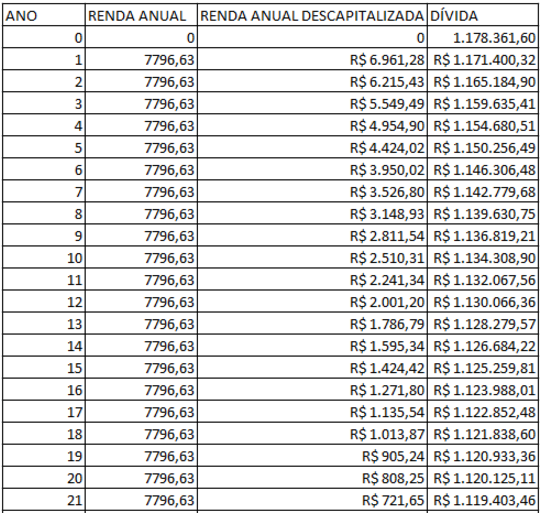
\includegraphics[width=.5\textwidth]{figuras/payback.png}
\caption{Planilha de Cálculo do Payback}
\label{fig:payback}
\end{figure}

Podemos observar que em 21 anos, o projeto ainda não se pagará, configurando assim, uma inviabilidade econômica. 

Se for possível dobrar a quantidade de placas solares e receber dejetos de pequenos produtores e da população da cidade do Gama, dobraremos a geração de energia elétrica, tornando assim o projeto mais viável. 
